\documentclass[11pt,a4paper]{article}
\usepackage[utf8]{inputenc}
\usepackage[T1]{fontenc}
\usepackage{graphicx}
\usepackage{listings}
\usepackage{xcolor}
\usepackage{hyperref}
\usepackage{amsmath}
\usepackage{amssymb}
\usepackage{tikz}
\usepackage{geometry}
\usetikzlibrary{arrows.meta,positioning}
\geometry{margin=1in}

\definecolor{codegreen}{rgb}{0,0.6,0}
\definecolor{codegray}{rgb}{0.5,0.5,0.5}
\definecolor{codepurple}{rgb}{0.58,0,0.82}
\definecolor{backcolour}{rgb}{0.95,0.95,0.92}

\lstdefinestyle{coursestyle}{
    backgroundcolor=\color{backcolour},
    commentstyle=\color{codegreen},
    keywordstyle=\color{magenta},
    numberstyle=\tiny\color{codegray},
    stringstyle=\color{codepurple},
    basicstyle=\ttfamily\small,
    breakatwhitespace=false,
    breaklines=true,
    captionpos=b,
    keepspaces=true,
    numbers=left,
    numbersep=5pt,
    showspaces=false,
    showstringspaces=false,
    showtabs=false,
    tabsize=2
}

\lstset{style=coursestyle}

\title{Learn IREE:\\
A Beginner Course on MLIR-Based Compilation and Runtime}
\author{Djordje Todorovic}
\date{March 2026}

\begin{document}

\maketitle

\tableofcontents
\newpage

\section{Preface}

This course is a beginner-friendly introduction to IREE: the Intermediate Representation Execution Environment. It is written for engineers who already know some Python, C/C++, or ML tooling, but who are new to compiler pipelines and runtime systems.

The goal is not to turn you into an IREE core maintainer in one sitting. The goal is to give you a solid mental model, enough vocabulary to read the code and documentation, and enough hands-on examples to compile and run small programs without guessing.

\subsection{Who This Course Is For}

This material is a good fit if you are:
\begin{itemize}
    \item an ML engineer who wants to understand what happens after model export,
    \item a compiler beginner who already knows what MLIR is at a high level,
    \item a systems engineer exploring runtimes, target backends, and hardware abstraction layers,
    \item a student who wants a practical entry point instead of a purely theoretical overview.
\end{itemize}

\subsection{Prerequisites}

You should be comfortable with:
\begin{itemize}
    \item command-line work on Linux or macOS,
    \item basic programming concepts such as functions, types, and modules,
    \item the rough idea that machine learning programs operate on tensors.
\end{itemize}

You do \textbf{not} need to know the internals of LLVM, MLIR, or GPU drivers before starting.

\subsection{Version Note}

IREE changes quickly. The commands and package names in this course were aligned with the official IREE documentation available on March 9, 2026. If a command behaves differently on your checkout, first run \texttt{iree-compile --help} or \texttt{iree-run-module --help}, then compare with the current docs.

\section{What IREE Is and Why It Exists}

IREE is an MLIR-based compiler and runtime for deploying tensor programs across different kinds of hardware. The simplest mental model is:

\begin{quote}
Take a model or MLIR program, lower it through several compiler stages, package the result into a deployable module, and execute it through a small runtime that talks to a real device.
\end{quote}

That device may be:
\begin{itemize}
    \item a CPU,
    \item a GPU through Vulkan, CUDA, HIP, or Metal,
    \item a reference backend such as \texttt{vmvx},
    \item or a custom accelerator integrated through IREE's compiler and runtime extension points.
\end{itemize}

\subsection{Why People Use IREE}

IREE is useful because it gives you one compiler and one runtime framework for many deployment targets. That matters when you want:
\begin{itemize}
    \item one toolchain across CPU, GPU, and accelerator targets,
    \item ahead-of-time compilation into deployable artifacts,
    \item small runtime footprints,
    \item clear separation between compilation and execution,
    \item a compiler pipeline built on top of MLIR instead of opaque framework internals.
\end{itemize}

\subsection{What IREE Is Not}

IREE is not:
\begin{itemize}
    \item a training framework,
    \item a replacement for PyTorch, JAX, or TensorFlow authoring,
    \item a single monolithic backend with one hard-coded target.
\end{itemize}

It sits later in the stack. You author a program elsewhere, then hand it to IREE in a supported input form.

\section{The Big Picture}

\subsection{End-to-End Pipeline}

At a high level, the IREE flow looks like this:

\begin{lstlisting}[caption=High-level IREE pipeline]
Frameworks / frontends
  PyTorch, JAX, TensorFlow, ONNX, StableHLO, MLIR
            |
            v
        Import / export
            |
            v
        Input MLIR
            |
            v
  IREE compiler pipeline
    ABI -> preprocessing -> optimization
    -> flow -> stream -> hal -> vm
            |
            v
      VMFB deployable artifact
            |
            v
        IREE runtime
            |
            v
 HAL driver + executable loader + device
            |
            v
       Target hardware
\end{lstlisting}

\subsection{A Visual Mental Model}

\begin{figure}[htbp]
\centering
\resizebox{0.98\textwidth}{!}{%
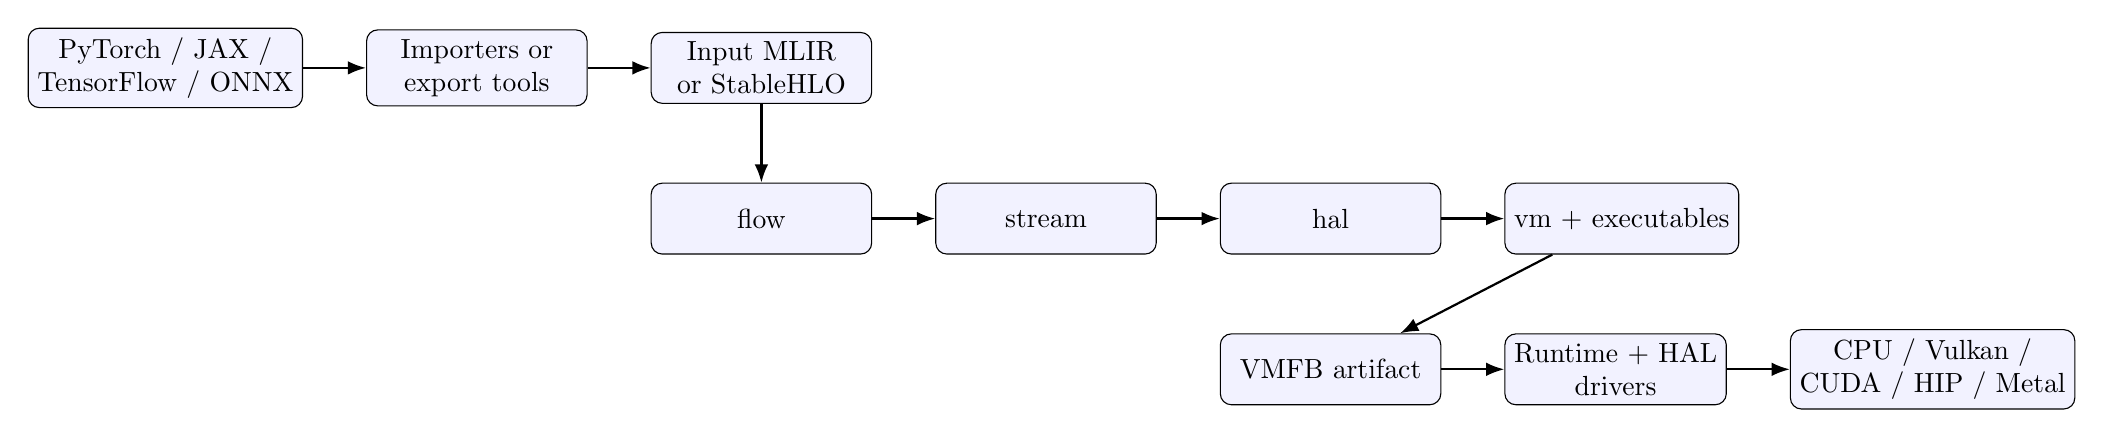
\begin{tikzpicture}[
  node distance=10mm and 8mm,
  box/.style={draw, rounded corners, align=center, minimum width=28mm, minimum height=9mm, fill=blue!5},
  arrow/.style={-Latex, thick}
]
\node[box] (frameworks) {PyTorch / JAX /\\TensorFlow / ONNX};
\node[box, right=of frameworks] (importers) {Importers or\\export tools};
\node[box, right=of importers] (inputmlir) {Input MLIR\\or StableHLO};
\node[box, below=of inputmlir] (flow) {flow};
\node[box, right=of flow] (stream) {stream};
\node[box, right=of stream] (hal) {hal};
\node[box, right=of hal] (vm) {vm + executables};
\node[box, below=of hal] (vmfb) {VMFB artifact};
\node[box, right=of vmfb] (runtime) {Runtime + HAL\\drivers};
\node[box, right=of runtime] (device) {CPU / Vulkan /\\CUDA / HIP / Metal};

\draw[arrow] (frameworks) -- (importers);
\draw[arrow] (importers) -- (inputmlir);
\draw[arrow] (inputmlir) -- (flow);
\draw[arrow] (flow) -- (stream);
\draw[arrow] (stream) -- (hal);
\draw[arrow] (hal) -- (vm);
\draw[arrow] (vm) -- (vmfb);
\draw[arrow] (vmfb) -- (runtime);
\draw[arrow] (runtime) -- (device);
\end{tikzpicture}
}
\caption{A beginner-friendly view of the IREE compiler and runtime stack.}
\end{figure}

\subsection{The Most Important Idea}

The most important idea in IREE is that \textbf{compilation and execution are separate concerns}.

\begin{itemize}
    \item The \textbf{compiler} lowers high-level tensor programs into deployable artifacts.
    \item The \textbf{runtime} loads those artifacts, allocates buffers, dispatches work, and synchronizes with devices.
\end{itemize}

Once this clicks, many IREE terms become easier to place.

\section{Core Vocabulary}

\begin{description}
    \item[MLIR] Multi-Level Intermediate Representation. The compiler infrastructure IREE builds on.
    \item[Dialect] A family of operations and types inside MLIR. Examples in IREE include \texttt{flow}, \texttt{stream}, \texttt{hal}, and \texttt{vm}.
    \item[Target backend] The code generation backend selected at compile time, such as \texttt{llvm-cpu}, \texttt{vmvx}, \texttt{vulkan-spirv}, or \texttt{cuda}.
    \item[Runtime driver] The runtime component that can actually execute compiled code on a device, such as \texttt{local-task}, \texttt{local-sync}, \texttt{vulkan}, or \texttt{cuda}.
    \item[VMFB] A FlatBuffer file containing an IREE deployable module plus metadata and executable payloads.
    \item[Dispatch] A unit of executable work handed to a device.
    \item[HAL] Hardware Abstraction Layer. The layer that hides device-specific details behind a common interface.
\end{description}

\section{How IREE Relates to MLIR and xDSL}

This repository already contains xDSL material, so it helps to place IREE relative to both MLIR and xDSL.

\subsection{MLIR, xDSL, and IREE in One View}

\begin{itemize}
    \item \textbf{MLIR} is the compiler infrastructure and IR framework.
    \item \textbf{xDSL} is a Python-native infrastructure inspired by MLIR and useful for learning, prototyping, and experimenting with compiler ideas.
    \item \textbf{IREE} is a production-oriented compiler and runtime stack built on MLIR for deploying tensor programs.
\end{itemize}

\subsection{A Useful Mental Separation}

\begin{description}
    \item[xDSL mindset] Build and understand compiler ideas quickly, often in Python, with explicit IR objects and passes you can inspect easily.
    \item[IREE mindset] Take a real tensor program, lower it through a serious deployment pipeline, package it, and execute it on actual hardware through a runtime.
\end{description}

\subsection{Why This Matters for Learning}

If you already understand xDSL's representation-and-transformation model, you have a good base for reading IREE:
\begin{itemize}
    \item both rely on explicit IR,
    \item both reward inspecting intermediate states,
    \item both make passes and dialect boundaries visible.
\end{itemize}

The difference is mainly \textbf{scope}. xDSL is excellent for learning and experimentation. IREE continues from those compiler ideas into concrete deployment and runtime execution.

\section{Compiler Stages You Should Recognize}

You do not need to master every pass name on day one. You should, however, know what the major stages are for.

\subsection{\texttt{flow}}

The \texttt{flow} dialect models tensor program data flow and partitions work into dispatchable regions. A useful mental shortcut is:

\begin{quote}
\texttt{flow} decides what chunks of tensor work should become executable dispatches.
\end{quote}

\subsection{\texttt{stream}}

The \texttt{stream} dialect models placement, asynchronous execution, and resource lifetimes. This is where the program becomes much more explicitly scheduled.

\begin{quote}
\texttt{stream} decides when work runs, where it runs, and how resources move through the schedule.
\end{quote}

\subsection{\texttt{hal}}

The \texttt{hal} dialect represents operations against IREE's hardware abstraction layer.

\begin{quote}
\texttt{hal} is where scheduling logic is expressed in a form that maps closely to the runtime API.
\end{quote}

\subsection{\texttt{vm}}

The \texttt{vm} layer represents IREE virtual machine code and module structure. By the end of compilation, you are close to the deployable representation that the runtime will load.

\section{Setting Up IREE}

\subsection{Build from Source}

If you are studying IREE itself, building from source is the best path because it gives you the compiler tools, the runtime, and the source tree in one place.

\subsubsection{Prerequisites}

For a typical Linux setup, the official docs recommend:
\begin{itemize}
    \item \texttt{cmake},
    \item \texttt{ninja},
    \item \texttt{clang},
    \item \texttt{lld}.
\end{itemize}

On Debian or Ubuntu:

\begin{lstlisting}[caption=Typical Linux prerequisites]
sudo apt install cmake ninja-build clang lld
\end{lstlisting}

\subsubsection{Clone and Configure}

\begin{lstlisting}[caption=Clone and configure IREE]
git clone https://github.com/iree-org/iree.git
cd iree
git submodule update --init

cmake -G Ninja -B ../iree-build/ -S . \
  -DCMAKE_BUILD_TYPE=RelWithDebInfo \
  -DIREE_ENABLE_ASSERTIONS=ON \
  -DIREE_ENABLE_SPLIT_DWARF=ON \
  -DIREE_ENABLE_THIN_ARCHIVES=ON \
  -DCMAKE_C_COMPILER=clang \
  -DCMAKE_CXX_COMPILER=clang++ \
  -DIREE_ENABLE_LLD=ON
\end{lstlisting}

\subsubsection{Build the Developer Tools}

\begin{lstlisting}[caption=Build a minimal useful tool set]
cmake --build ../iree-build/ \
  --target iree-compile iree-run-module iree-benchmark-module \
           iree-dump-module iree-opt iree-check-module
\end{lstlisting}

This course uses those tools constantly.

\subsubsection{Run the Test Suite}

\begin{lstlisting}[caption=Run the CMake test wrapper]
./build_tools/cmake/ctest_all.sh ../iree-build
\end{lstlisting}

\subsection{Python Packages}

If you only need the packaged compiler and runtime, the current package names are:
\begin{itemize}
    \item \texttt{iree-base-compiler}
    \item \texttt{iree-base-runtime}
\end{itemize}

The older package names \texttt{iree-compiler} and \texttt{iree-runtime} are deprecated.

\begin{lstlisting}[caption=Install the packaged compiler and runtime]
python -m pip install iree-base-compiler iree-base-runtime
\end{lstlisting}

\section{Meet the Main Tools}

\begin{tabular}{|l|p{9cm}|}
\hline
\textbf{Tool} & \textbf{What it does} \\
\hline
\texttt{iree-compile} & Compiles supported MLIR input into a deployable IREE module. \\
\hline
\texttt{iree-run-module} & Loads a compiled module and invokes an exported function. \\
\hline
\texttt{iree-benchmark-module} & Benchmarks module execution with the same style of inputs as \texttt{iree-run-module}. \\
\hline
\texttt{iree-dump-module} & Prints the contents of a \texttt{.vmfb} module. \\
\hline
\texttt{iree-opt} & Runs selected compiler passes and transformation pipelines on MLIR. \\
\hline
\texttt{iree-check-module} & Runs check-style tests embedded in compiled modules. \\
\hline
\texttt{iree-run-mlir} & Compiles and runs an MLIR file directly for testing and debugging. \\
\hline
\end{tabular}

\section{How To Read an IREE Command Line}

One reason IREE feels difficult at first is that the commands are dense. They become much easier once you read them as answers to a few fixed questions.

\subsection{Reading a Compile Command}

Consider this example:

\begin{lstlisting}[caption=An annotated compile command]
iree-compile \
  --iree-hal-target-device=local \
  --iree-hal-local-target-device-backends=llvm-cpu \
  --iree-llvmcpu-target-cpu=host \
  simple_abs.mlir \
  -o simple_abs_cpu.vmfb
\end{lstlisting}

Read it like this:
\begin{enumerate}
    \item \textbf{What is the input?} \texttt{simple\_abs.mlir}
    \item \textbf{What device family am I targeting?} \texttt{local}
    \item \textbf{What executable backend do I want?} \texttt{llvm-cpu}
    \item \textbf{How should CPU code be tuned?} \texttt{host}
    \item \textbf{Where does the artifact go?} \texttt{simple\_abs\_cpu.vmfb}
\end{enumerate}

\subsection{Reading a Run Command}

Now consider the matching runtime command:

\begin{lstlisting}[caption=An annotated run command]
iree-run-module \
  --module=simple_abs_cpu.vmfb \
  --device=local-task \
  --function=abs \
  --input=f32=-2
\end{lstlisting}

Read it like this:
\begin{enumerate}
    \item \textbf{What module am I loading?}
    \item \textbf{What runtime device should execute it?}
    \item \textbf{What exported function should be called?}
    \item \textbf{What inputs should be passed?}
\end{enumerate}

\subsection{The Two Questions Beginners Mix Up}

Do not confuse these:
\begin{itemize}
    \item \texttt{--iree-hal-local-target-device-backends=llvm-cpu}: compile-time code generation choice.
    \item \texttt{--device=local-task}: runtime execution device choice.
\end{itemize}

The first changes what gets emitted. The second changes how the already-compiled module is executed.

\subsection{A Tiny Backend Cheat Sheet}

\begin{tabular}{|l|p{3.1cm}|p{6cm}|}
\hline
\textbf{Backend} & \textbf{Good first use} & \textbf{Beginner note} \\
\hline
\texttt{vmvx} & Reference execution and learning & Simple and portable, but not the fast path. \\
\hline
\texttt{llvm-cpu} & Real CPU deployment & Usually pair with \texttt{--iree-llvmcpu-target-cpu=host}. \\
\hline
\texttt{vulkan-spirv} & Vulkan-capable GPUs & Requires a working Vulkan runtime stack. \\
\hline
\texttt{cuda} & NVIDIA GPUs & Runtime device must also support CUDA. \\
\hline
\texttt{rocm} or \texttt{hip} & AMD GPUs & Platform-specific setup matters. \\
\hline
\end{tabular}

\section{Your First IREE Program}

We will start with a tiny MLIR program that computes an absolute value.

\subsection{Step 1: Write \texttt{simple\_abs.mlir}}

\begin{lstlisting}[caption=A minimal IREE-friendly MLIR example]
module {
  func.func @abs(%arg0: tensor<f32>) -> tensor<f32> {
    %0 = math.absf %arg0 : tensor<f32>
    return %0 : tensor<f32>
  }
}
\end{lstlisting}

\subsection{Step 2: Compile It to \texttt{vmvx}}

For a first run, \texttt{vmvx} is a nice backend because it is simple and portable. It is not the fast path, but it is a good learning path.

\begin{lstlisting}[caption=Compile the program to a VMFB using VMVX]
iree-compile \
  --iree-hal-target-device=local \
  --iree-hal-local-target-device-backends=vmvx \
  simple_abs.mlir \
  -o simple_abs_vmvx.vmfb
\end{lstlisting}

\subsection{Step 3: Run It}

\begin{lstlisting}[caption=Execute the exported function]
iree-run-module \
  --module=simple_abs_vmvx.vmfb \
  --device=local-task \
  --function=abs \
  --input=f32=-2
\end{lstlisting}

You should see a result equivalent to:

\begin{lstlisting}[caption=Expected shape of the output]
EXEC @abs
result[0]: hal.buffer_view
f32=2
\end{lstlisting}

\subsection{What Just Happened}

\begin{enumerate}
    \item \texttt{iree-compile} lowered your MLIR into IREE's internal pipeline.
    \item It emitted a \texttt{.vmfb} module.
    \item \texttt{iree-run-module} loaded that module.
    \item The runtime selected the \texttt{local-task} CPU device.
    \item The exported function \texttt{abs} was invoked with one scalar tensor input.
\end{enumerate}

\subsection{Shortcut for Experimentation}

If you want a quick feedback loop while learning, you can skip the explicit \texttt{.vmfb} file and run the MLIR file directly:

\begin{lstlisting}[caption=Compile and run directly from MLIR]
iree-run-mlir \
  --iree-hal-target-device=local \
  --iree-hal-local-target-device-backends=vmvx \
  simple_abs.mlir \
  --function=abs \
  --input=f32=-2
\end{lstlisting}

\section{Running on CPU the Usual Way}

For real CPU execution you will usually target \texttt{llvm-cpu}, not \texttt{vmvx}.

\subsection{Compile for \texttt{llvm-cpu}}

\begin{lstlisting}[caption=Compile for host CPU execution]
iree-compile \
  --iree-hal-target-device=local \
  --iree-hal-local-target-device-backends=llvm-cpu \
  --iree-llvmcpu-target-cpu=host \
  --iree-opt-level=O2 \
  simple_abs.mlir \
  -o simple_abs_cpu.vmfb
\end{lstlisting}

Two flags matter here:
\begin{itemize}
    \item \texttt{--iree-hal-local-target-device-backends=llvm-cpu}: use LLVM CPU code generation.
    \item \texttt{--iree-llvmcpu-target-cpu=host}: optimize for the machine you are compiling on.
\end{itemize}

If you omit the target CPU, IREE may fall back to a generic CPU target, which is easier to run everywhere but usually slower.

\subsection{Run It}

\begin{lstlisting}[caption=Run the CPU-targeted module]
iree-run-module \
  --module=simple_abs_cpu.vmfb \
  --device=local-task \
  --function=abs \
  --input=f32=-2
\end{lstlisting}

\subsection{Check Available Drivers and Devices}

\begin{lstlisting}[caption=Inspect what the runtime can see]
iree-run-module --list_drivers
iree-run-module --list_devices
\end{lstlisting}

For CPU work you should expect to see \texttt{local-sync://} and \texttt{local-task://}.

\subsection{\texttt{local-sync} vs \texttt{local-task}}

\begin{description}
    \item[\texttt{local-sync}] Synchronous, single-threaded, easier to follow in a debugger.
    \item[\texttt{local-task}] Asynchronous, multithreaded, closer to typical production CPU execution.
\end{description}

When learning runtime internals, start with \texttt{local-sync}. When measuring ordinary CPU execution, use \texttt{local-task}.

\section{Small Example 2: Scale a Vector}

The first example used a scalar tensor. Now let us run something slightly more realistic.

\subsection{Write \texttt{scale\_by\_two.mlir}}

\begin{lstlisting}[caption=A tiny vector example]
module {
  func.func @scale_by_two(%arg0: tensor<4xf32>) -> tensor<4xf32> {
    %cst = arith.constant dense<2.0> : tensor<4xf32>
    %0 = arith.mulf %arg0, %cst : tensor<4xf32>
    return %0 : tensor<4xf32>
  }
}
\end{lstlisting}

\subsection{Compile and Run}

\begin{lstlisting}[caption=Compile and execute the vector example]
iree-compile \
  --iree-hal-target-device=local \
  --iree-hal-local-target-device-backends=llvm-cpu \
  --iree-llvmcpu-target-cpu=host \
  scale_by_two.mlir \
  -o scale_by_two.vmfb

iree-run-module \
  --module=scale_by_two.vmfb \
  --device=local-task \
  --function=scale_by_two \
  --input="4xf32=1 -3 0.5 -2"
\end{lstlisting}

Expected output:

\begin{lstlisting}[caption=Expected output]
EXEC @scale_by_two
result[0]: hal.buffer_view
4xf32=2 -6 1 -4
\end{lstlisting}

\subsection{Why This Example Matters}

This small program introduces three useful habits:
\begin{itemize}
    \item reading tensor input syntax,
    \item thinking about exported function signatures,
    \item separating the compiler target backend from the runtime device selection.
\end{itemize}

\section{How \texttt{iree-run-module} Inputs Work}

The input format is simple once you have seen a few examples.

\begin{tabular}{|l|p{8cm}|}
\hline
\textbf{MLIR type} & \textbf{Example flag} \\
\hline
\texttt{i32} & \texttt{--input=1234} \\
\hline
\texttt{tensor<i32>} & \texttt{--input=i32=1234} \\
\hline
\texttt{tensor<2xi32>} & \texttt{--input="2xi32=12 34"} \\
\hline
\texttt{tensor<2x3xi32>} & \texttt{--input="2x3xi32=[1 2 3][4 5 6]"} \\
\hline
\end{tabular}

\subsection{Practical Advice}

\begin{itemize}
    \item Quote inputs that contain spaces.
    \item Match the function signature exactly.
    \item If you are unsure what the function expects, inspect the source MLIR or dump the compiled module.
    \item Inputs can also be loaded from raw binary files or NumPy \texttt{.npy} files.
\end{itemize}

\section{Learning the Pipeline by Dumping Phases}

One of the best beginner techniques in IREE is to dump the IR after each compiler phase and compare the files.

\subsection{Dump All Compilation Phases}

\begin{lstlisting}[caption=Dump the pipeline step by step]
mkdir -p /tmp/iree/simple_abs

iree-compile simple_abs.mlir \
  --iree-hal-target-device=local \
  --iree-hal-local-target-device-backends=llvm-cpu \
  --iree-llvmcpu-target-cpu=host \
  --dump-compilation-phases-to=/tmp/iree/simple_abs \
  -o /tmp/iree/simple_abs/simple_abs_cpu.vmfb
\end{lstlisting}

You should get files with names shaped like:

\begin{lstlisting}[caption=Typical dumped phase files]
simple_abs.1.input.mlir
simple_abs.2.abi.mlir
simple_abs.3.preprocessing.mlir
simple_abs.4.global-optimization.mlir
simple_abs.5.dispatch-creation.mlir
simple_abs.6.flow.mlir
simple_abs.7.stream.mlir
simple_abs.8.executable-sources.mlir
simple_abs.9.executable-configurations.mlir
simple_abs.10.executable-targets.mlir
simple_abs.11.hal.mlir
simple_abs.12.vm.mlir
\end{lstlisting}

\subsection{How To Read Them}

\begin{description}
    \item[\texttt{input}] Your starting point.
    \item[\texttt{abi}] Entry-point and calling-convention shaping.
    \item[\texttt{preprocessing}] Canonical cleanup and early normalization.
    \item[\texttt{global-optimization}] Whole-program simplifications.
    \item[\texttt{dispatch-creation}] Compute regions become explicit dispatch candidates.
    \item[\texttt{flow}] Tensor work is organized as dispatchable data flow.
    \item[\texttt{stream}] Scheduling and resource management become more explicit.
    \item[\texttt{hal}] The program is expressed in terms of device-facing runtime concepts.
    \item[\texttt{vm}] The final VM-oriented representation before packaging.
\end{description}

\subsection{Why This Is So Valuable}

If you come from xDSL or general MLIR learning, this is the closest thing to a live anatomy lesson for IREE. Instead of memorizing names, you can watch the same program become progressively lower level.

\section{HAL for Beginners}

HAL is one of the most important concepts in IREE, and it is also one of the most misunderstood.

\subsection{What HAL Is}

HAL stands for Hardware Abstraction Layer. It is the layer between the runtime and actual hardware-specific implementations.

HAL exists in two related forms:
\begin{itemize}
    \item a \textbf{compile-time MLIR dialect} named \texttt{hal},
    \item a \textbf{runtime API and driver interface} implemented in the runtime.
\end{itemize}

\subsection{Compile-Time HAL}

At compile time, HAL is used to express operations such as:
\begin{itemize}
    \item device interaction,
    \item buffer management,
    \item executable packaging,
    \item synchronization and dispatch structure.
\end{itemize}

The important beginner point is this:

\begin{quote}
IREE does not use HAL to represent the math itself. It uses HAL to represent how compiled work is prepared and executed on devices.
\end{quote}

\subsection{Runtime HAL}

At runtime, HAL drivers implement the abstract operations required by the compiler output. That includes things like:
\begin{itemize}
    \item buffer allocation,
    \item command submission,
    \item fences and semaphores,
    \item loading executable payloads,
    \item device enumeration.
\end{itemize}

\subsection{Target Backend vs Runtime Driver}

This distinction matters:

\begin{itemize}
    \item \textbf{Target backend}: compile-time code generation choice.
    \item \textbf{Runtime driver}: execution-time device interface.
\end{itemize}

Examples:
\begin{itemize}
    \item \texttt{llvm-cpu} is a compiler backend.
    \item \texttt{local-task} and \texttt{local-sync} are runtime drivers/devices for CPU execution.
    \item \texttt{vulkan-spirv} is a compiler backend.
    \item \texttt{vulkan} is the runtime driver.
\end{itemize}

If you mix these up, many IREE command lines stop making sense.

\section{Runtime Building Blocks}

Once you move past the first few CLI examples, the runtime becomes much easier to understand if you know its core objects.

\subsection{Driver}

The driver is the top-level runtime entry point for a device family. It is responsible for discovering devices and creating device instances.

\begin{quote}
Think of the driver as the runtime-side bridge between ``I know I want Vulkan or local CPU'' and ``give me an actual device object I can use''.
\end{quote}

\subsection{Device}

The device is the execution surface. Command buffers are submitted to devices, buffers are allocated through device-associated allocators, and synchronization is observed at this level.

For beginners, the most visible devices are:
\begin{itemize}
    \item \texttt{local-sync}
    \item \texttt{local-task}
    \item GPU-facing devices such as \texttt{vulkan} or \texttt{cuda}
\end{itemize}

\subsection{Allocator and Buffers}

Tensor data eventually lives in buffers managed by HAL allocators. A buffer may live in host-visible memory, device-local memory, or some combination depending on the backend.

This matters because a lot of ``why is this runtime code so large?'' questions reduce to:
\begin{itemize}
    \item where does the data live,
    \item who is allowed to see it,
    \item when is movement or mapping required.
\end{itemize}

\subsection{Command Buffer}

A command buffer records work to be executed later. In IREE this includes dispatches, transfers, and synchronization-related operations.

If you have seen Vulkan before, this concept should feel familiar. If not, use this shortcut:

\begin{quote}
A command buffer is a recorded plan for device work, not the work itself.
\end{quote}

\subsection{Executable}

An executable is the compiled device-facing payload. It may come from LLVM CPU code generation, SPIR-V, CUDA-related lowering, or other backend-specific formats.

The runtime does not ``re-derive'' the math from scratch. It loads executable payloads that the compiler already produced.

\subsection{Semaphores and Fences}

These are synchronization tools:
\begin{itemize}
    \item \textbf{semaphores} coordinate ordering across submissions and device work,
    \item \textbf{fences} help coordinate between host and device completion points.
\end{itemize}

You do not need to implement them to benefit from them. You only need to understand that correct execution on asynchronous systems requires explicit ordering.

\subsection{Why This Section Matters}

When you later read files under \texttt{runtime/src/iree/hal/}, you will keep seeing the same nouns: driver, device, allocator, command buffer, executable, semaphore. Learning those nouns early makes the runtime code much less intimidating.

\section{VMFB and IREE Modules}

\subsection{What a VMFB Is}

A \texttt{.vmfb} file is an IREE module packaged in FlatBuffer form. It typically contains:
\begin{itemize}
    \item VM bytecode and metadata,
    \item references to required runtime modules,
    \item executable payloads for one or more targets,
    \item exported function information.
\end{itemize}

\subsection{Inspect a Module}

\begin{lstlisting}[caption=Inspect a VMFB]
iree-dump-module simple_abs_cpu.vmfb
\end{lstlisting}

You will see information such as:
\begin{itemize}
    \item required types,
    \item module dependencies,
    \item imported functions,
    \item exported functions.
\end{itemize}

This is a very useful habit when you are unsure whether a function is really exported or what runtime modules the artifact expects.

\subsection{A Useful Mental Model}

Many beginners imagine that a program is just one blob of machine code. In IREE, it is better to think in terms of \textbf{modules plus executables plus runtime services}. The VM coordinates modules. The HAL handles device-facing work. The executable payloads do the dense compute.

\section{Small How-To 1: Benchmark a Module}

After you can compile and run a program once, the next useful step is to benchmark it.

\begin{lstlisting}[caption=Benchmark the same exported function]
iree-benchmark-module \
  --module=simple_abs_cpu.vmfb \
  --device=local-task \
  --function=abs \
  --input=f32=-2
\end{lstlisting}

This measures full module invocation overhead, including VM and runtime activity, not just one raw kernel in isolation.

\section{Small How-To 2: Dump Executable Files}

If you want to see what device-specific code was generated, ask the compiler to dump executable-related files.

\begin{lstlisting}[caption=Dump generated executable artifacts]
mkdir -p /tmp/iree/simple_abs_dump

iree-compile simple_abs.mlir \
  --iree-hal-target-device=local \
  --iree-hal-local-target-device-backends=llvm-cpu \
  --iree-llvmcpu-link-embedded=false \
  --iree-hal-dump-executable-files-to=/tmp/iree/simple_abs_dump \
  -o /tmp/iree/simple_abs_dump/simple_abs_cpu.vmfb
\end{lstlisting}

You may see files such as:
\begin{itemize}
    \item \texttt{module\_abs\_dispatch\_0.mlir},
    \item \texttt{module\_abs\_dispatch\_0\_system\_elf\_x86\_64.codegen.ll},
    \item \texttt{module\_abs\_dispatch\_0\_system\_elf\_x86\_64.o},
    \item \texttt{module\_abs\_dispatch\_0\_system\_elf\_x86\_64.so}.
\end{itemize}

This is where the compiler stops feeling abstract. You can literally inspect the generated dispatch sources and target-specific binaries.

\section{Small How-To 3: Isolate a Dispatch Benchmark}

The compiler can also dump benchmarkable dispatch modules.

\begin{lstlisting}[caption=Generate and benchmark a single dispatch module]
iree-compile simple_abs.mlir \
  --iree-hal-target-device=local \
  --iree-hal-local-target-device-backends=llvm-cpu \
  --iree-hal-dump-executable-benchmarks-to=/tmp/iree/simple_abs_bench \
  -o /dev/null

iree-compile \
  /tmp/iree/simple_abs_bench/module_abs_dispatch_0_embedded_elf_x86_64_benchmark.mlir \
  -o /tmp/iree/simple_abs_bench/module_abs_dispatch_0_benchmark.vmfb

iree-benchmark-module \
  --module=/tmp/iree/simple_abs_bench/module_abs_dispatch_0_benchmark.vmfb
\end{lstlisting}

This is useful when you want to understand the performance of one dispatch without all surrounding application logic.
These generated benchmark modules use fake buffers and synthetic operands, so treat them as a starting point for investigation, not as a substitute for a real end-to-end benchmark.

\section{Small How-To 4: Import an ONNX Model}

For a beginner course it is enough to understand the shape of the workflow.

\begin{lstlisting}[caption=Import ONNX, compile, and run on CPU]
python -m pip install "iree-base-compiler[onnx]" iree-base-runtime

iree-import-onnx mobilenetv2-10.onnx --opset-version 17 -o mobilenetv2.mlir

iree-compile \
  --iree-hal-target-device=local \
  --iree-hal-local-target-device-backends=llvm-cpu \
  --iree-llvmcpu-target-cpu=host \
  --iree-opt-level=O2 \
  mobilenetv2.mlir \
  -o mobilenet_cpu.vmfb

iree-run-module \
  --module=mobilenet_cpu.vmfb \
  --device=local-task \
  --function=... \
  --input="1x3x224x224xf32=0"
\end{lstlisting}

The last two placeholders are model-specific:
\begin{itemize}
    \item the exported function name,
    \item the exact input signature.
\end{itemize}

If you are working from PyTorch instead of ONNX, the official PyTorch frontend is \texttt{iree-turbine}.

\section{Debugging}

\subsection{Use \texttt{local-sync} First}

When stepping through runtime execution, prefer \texttt{local-sync} because it avoids multithreaded scheduling noise.

\subsection{Debug \texttt{iree-run-module} with LLDB}

\begin{lstlisting}[caption=Launch the runtime under LLDB]
lldb -- ./iree-build/tools/iree-run-module \
  --module=simple_abs_cpu.vmfb \
  --device=local-sync \
  --function=abs \
  --input=f32=-2
\end{lstlisting}

Useful LLDB commands:
\begin{itemize}
    \item \texttt{break set -n function\_name}
    \item \texttt{break set -r iree\_hal.*}
    \item \texttt{run}
    \item \texttt{next}
    \item \texttt{step}
    \item \texttt{continue}
    \item \texttt{bt}
    \item \texttt{frame variable}
\end{itemize}

\subsection{GDB Alternative}

\begin{lstlisting}[caption=Launch the runtime under GDB]
gdb --args ./iree-build/tools/iree-run-module \
  --module=simple_abs_cpu.vmfb \
  --device=local-sync \
  --function=abs \
  --input=f32=-2
\end{lstlisting}

\subsection{Three Good Debug Habits}

\begin{enumerate}
    \item Dump the module with \texttt{iree-dump-module}.
    \item Dump compiler phases with \texttt{--dump-compilation-phases-to}.
    \item Switch from \texttt{local-task} to \texttt{local-sync} when you need a clearer execution story.
\end{enumerate}

\section{Troubleshooting Checklist}

When something fails in IREE, the fastest path is usually to classify the failure before changing random flags.

\begin{description}
    \item[``Device not found'' or ``driver not available''] Run \texttt{iree-run-module --list\_drivers} and \texttt{--list\_devices}. Confirm that your runtime was built with the driver you expect.
    \item[``Function not found''] Use \texttt{iree-dump-module} and verify the exported function name.
    \item[Shape or type mismatch] Compare your \texttt{--input=} flags against the function signature in the source MLIR or dumped module.
    \item[CPU result is correct but unexpectedly slow] Rebuild or recompile with \texttt{--iree-llvmcpu-target-cpu=host}. Also make sure you are not benchmarking \texttt{vmvx} by accident.
    \item[Execution is hard to follow] Switch from \texttt{local-task} to \texttt{local-sync} and rerun under a debugger.
    \item[Compiler pipeline feels opaque] Use \texttt{--dump-compilation-phases-to=} and compare \texttt{flow}, \texttt{stream}, \texttt{hal}, and \texttt{vm}.
\end{description}

\subsection{A Good Investigation Order}

For most beginner issues, this order works well:
\begin{enumerate}
    \item verify the source MLIR,
    \item compile with explicit backend flags,
    \item dump the module,
    \item run with explicit device selection,
    \item switch to \texttt{local-sync} if needed,
    \item only then start reading runtime internals.
\end{enumerate}

\section{Common Beginner Mistakes}

\begin{enumerate}
    \item \textbf{Confusing backend and device.} \texttt{llvm-cpu} is not a runtime device string; \texttt{local-task} is.
    \item \textbf{Forgetting to export or call the right function.} The runtime only sees exported functions.
    \item \textbf{Passing the wrong input shape.} Match the exact tensor shape and element type.
    \item \textbf{Using \texttt{vmvx} and expecting top CPU performance.} \texttt{vmvx} is primarily a reference backend.
    \item \textbf{Ignoring the target CPU flag.} On CPU, \texttt{--iree-llvmcpu-target-cpu=host} is often the right default when not cross-compiling.
    \item \textbf{Trying to learn everything at once.} First learn compile, run, inspect, and benchmark. Then read the lower-level runtime code.
\end{enumerate}

\section{A Beginner Reading Order for the Source Tree}

Once you are ready to inspect the IREE repository itself, this is a practical order:

\begin{enumerate}
    \item \texttt{samples/} to see small end-to-end examples,
    \item \texttt{tools/} to understand the CLI front doors,
    \item compiler dialect docs for \texttt{flow}, \texttt{stream}, \texttt{hal}, and \texttt{vm},
    \item \texttt{runtime/src/iree/hal/} for the HAL API and drivers,
    \item the CPU runtime drivers such as \texttt{local-sync} and \texttt{local-task}.
\end{enumerate}

\section{Glossary}

\begin{description}
    \item[ABI] Application Binary Interface. In IREE, this includes how entry points are shaped and called.
    \item[Bytecode module] A module containing VM bytecode interpreted by IREE's virtual machine.
    \item[Dispatch] A unit of scheduled executable work.
    \item[Executable] Target-specific compiled compute payload attached to a module.
    \item[HAL] Hardware Abstraction Layer used by the compiler and runtime.
    \item[Importer] A tool that converts a framework-specific program into a form IREE can compile.
    \item[MLIR] The compiler infrastructure beneath IREE.
    \item[Runtime driver] The execution-time implementation for a device family.
    \item[Stream] IREE dialect handling placement, scheduling, and resource lifetime modeling.
    \item[Target backend] The compile-time code generation backend.
    \item[VM] IREE's virtual machine layer.
    \item[VMFB] The deployable FlatBuffer container produced by the compiler.
    \item[VMVX] A portable reference executable backend used frequently in examples and testing.
\end{description}

\section{Exercises}

Try these in order:

\begin{enumerate}
    \item Compile \texttt{simple\_abs.mlir} to both \texttt{vmvx} and \texttt{llvm-cpu}. Compare the commands and outputs.
    \item Dump the compilation phases for \texttt{simple\_abs.mlir}. Open \texttt{simple\_abs.6.flow.mlir} and \texttt{simple\_abs.7.stream.mlir}. Write down the biggest structural difference you notice.
    \item Modify \texttt{scale\_by\_two.mlir} so it multiplies by \texttt{3.0} instead of \texttt{2.0}.
    \item Run the same module once with \texttt{local-sync} and once with \texttt{local-task}.
    \item Use \texttt{iree-dump-module} on a compiled VMFB and identify the exported function names.
    \item Import a tiny ONNX model and compile it for CPU.
\end{enumerate}

\section{Where To Go Next}

After this course, a good next step is one of these:
\begin{itemize}
    \item learn one frontend path in depth, such as ONNX or PyTorch through \texttt{iree-turbine},
    \item study the \texttt{flow -> stream -> hal} lowering path by diffing dumped phases,
    \item read the CPU deployment and benchmarking docs and start measuring real workloads,
    \item inspect the runtime HAL API and one concrete driver implementation.
\end{itemize}

\section{Official References}

These are the main official references that informed the practical commands in this course:

\begin{itemize}
    \item \href{https://iree.dev/building-from-source/getting-started/}{Getting Started}
    \item \href{https://iree.dev/developers/general/developer-overview/}{Developer Overview}
    \item \href{https://iree.dev/guides/deployment-configurations/cpu/}{CPU Deployment Guide}
    \item \href{https://iree.dev/developers/performance/benchmarking/}{Benchmarking}
    \item \href{https://iree.dev/developers/general/developer-tips/}{Developer Tips and Tricks}
    \item \href{https://iree.dev/reference/mlir-dialects/index.html}{IREE MLIR Dialects Reference}
\end{itemize}

\section{Closing Note}

If you remember only five things after the first pass through this material, remember these:
\begin{enumerate}
    \item IREE is both a compiler and a runtime.
    \item \texttt{flow}, \texttt{stream}, \texttt{hal}, and \texttt{vm} are the key pipeline names to recognize.
    \item \texttt{llvm-cpu} is a compile-time backend, while \texttt{local-task} and \texttt{local-sync} are runtime devices.
    \item \texttt{.vmfb} is the deployable module format you run.
    \item The fastest way to learn IREE is to compile, dump, inspect, and rerun tiny examples.
\end{enumerate}

\end{document}
